\chapter{Проектирование}

\section{Моделирование прямого цифрового синтеза}
Смоделируем алгоритм метода прямого цифрового синтеза на языке Си для дальнейшей реализации на микроконтроллере.

\begin{code}
\captionof{listing}{Метод DDS.}
\begin{minted}[mathescape,linenos,frame=lines,breaklines]{text}
  uint16_t p_acc, p_step;
  uint8_t addr = 0; // адрес ячейки

  p_acc = 0;    // аккумулятор фазы
  p_step = 256; // код частоты

  while (1) {
    addr = p_acc >> 8; // выделение старшей части аккумулятора фазы
    p_acc += p_step;   // шаг
    printf("%d 0x%X\n", addr, lut[addr]); // вывод отсчёта
}
\end{minted}
\end{code}

	Алгоритм программы представлен следующей блок-схемой.
	
\begin{figure}[H]
    \centering
    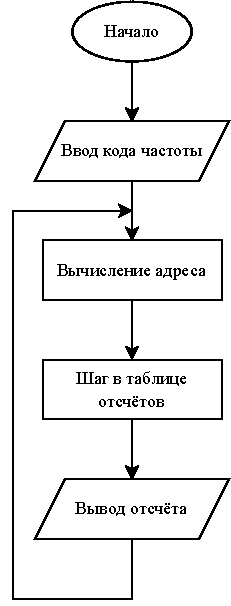
\includegraphics[width=0.3\textwidth]{../image/dds_block.pdf}
    \caption{Алгоритм метода DDS.}
\end{figure}
	
	Код частоты задаёт выходную частоту генератора. При значении 256 вывод будет следующий:
	
\begin{code}
\captionof{listing}{Формирование отсчётов при коде частоты 256.}
\begin{minted}[mathescape,linenos,frame=lines,breaklines]{text}
[kenny@desktop dds]\$ gcc dds.c -o dds && ./dds
0 0x7F
1 0x82
...
254 0x79
255 0x7C
\end{minted}
\end{code}
	
	Увеличим код частоты в два раза и получим следующее:

\begin{code}
\captionof{listing}{Формирование отсчётов при коде частоты 512.}
\begin{minted}[mathescape,linenos,frame=lines,breaklines]{text}
[kenny@desktop dds]\$ gcc dds.c -o dds && ./dds
0 0x7F
2 0x85
...
252 0x73
254 0x79
\end{minted}
\end{code}

	Как можно заметить отсчёты стали формироваться через один, соответственно частота вырастит в два раза. Теперь уменьшим частоту в два раза выставив код частоты 128.

\begin{code}
\captionof{listing}{Формирование отсчётов при коде частоты 128.}
\begin{minted}[mathescape,linenos,frame=lines,breaklines]{text}
[kenny@desktop dds]\$ gcc dds.c -o dds && ./dds
0 0x7F
0 0x7F
1 0x82
1 0x82
...
254 0x79
254 0x79
255 0x7C
255 0x7C
\end{minted}
\end{code}

	Программа стала выводить каждый отсчёт по два раза тем самым, понизив частоту.
	
	В данном виде модуляции код частоты просто абстрактное число, которое добавляется к аккумулятору фазы и узнать реальную частоту проблематично. Результат синтеза стоит проверить опытным путём на микроконтроллере.

\section{Алгоритм работы}


\section{Схема генератора}
\begin{figure}[h]
    \centering
    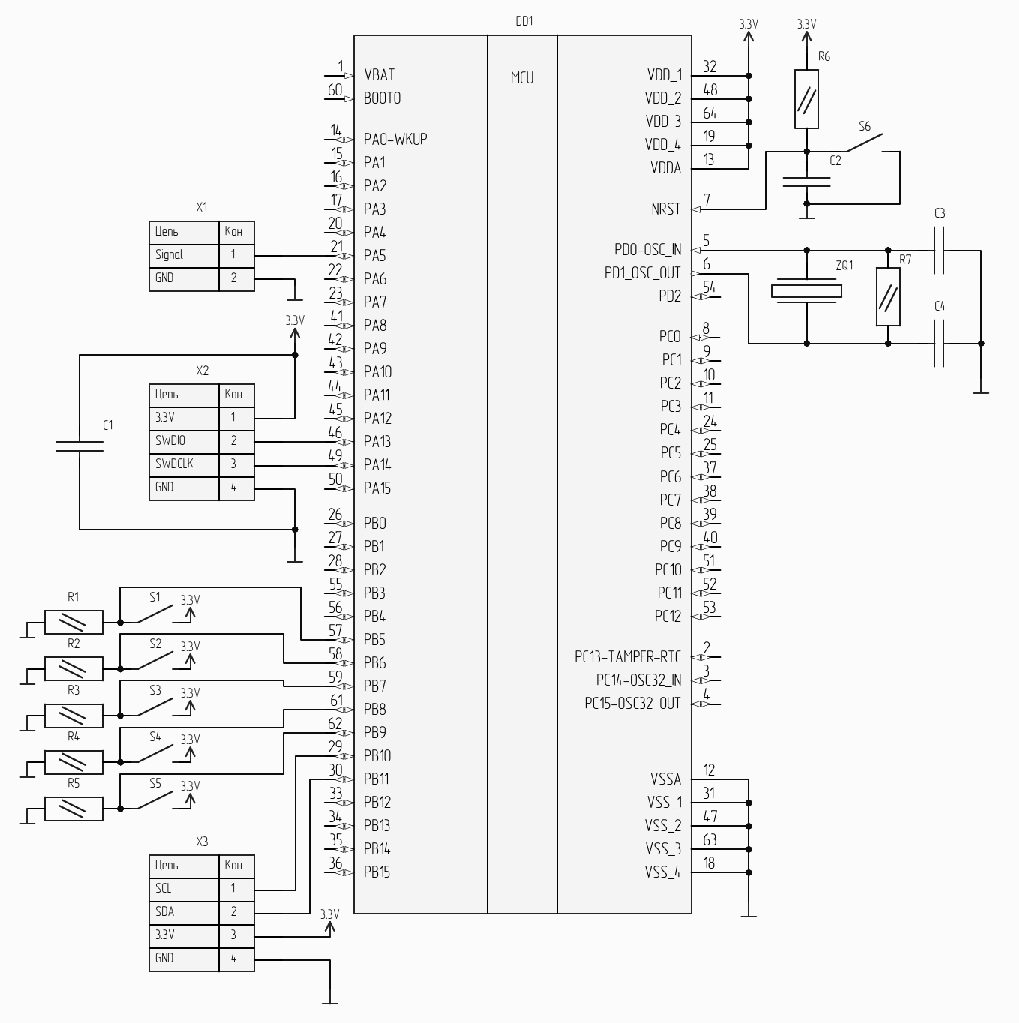
\includegraphics[width=1.0\textwidth]{../image/scheme-cropped.pdf}
    \caption{Схема электрическая принципиальная.}
\end{figure}

